\section{Implementation}\label{sec:impl}

The FFL runtime required an implementation that would translate specifications of augmentations to rendered HTML formulas. Figure~\ref{fig:dataflow} summarizes the translation process and the intermediate representations involved. Here, we briefly describe our implementation of augmentations in the FFL runtime in terms of each time the API is triggered.\footnote{\zed{Our implementation is hosted at \ifreview\textbf{[SEE CAMERA-READY VERSION]}\else\href{https://penn-hci.github.io/ffl}{\texttt{penn-hci.github.io/ffl}}\fi.}}

\begin{figure}
    \centering
    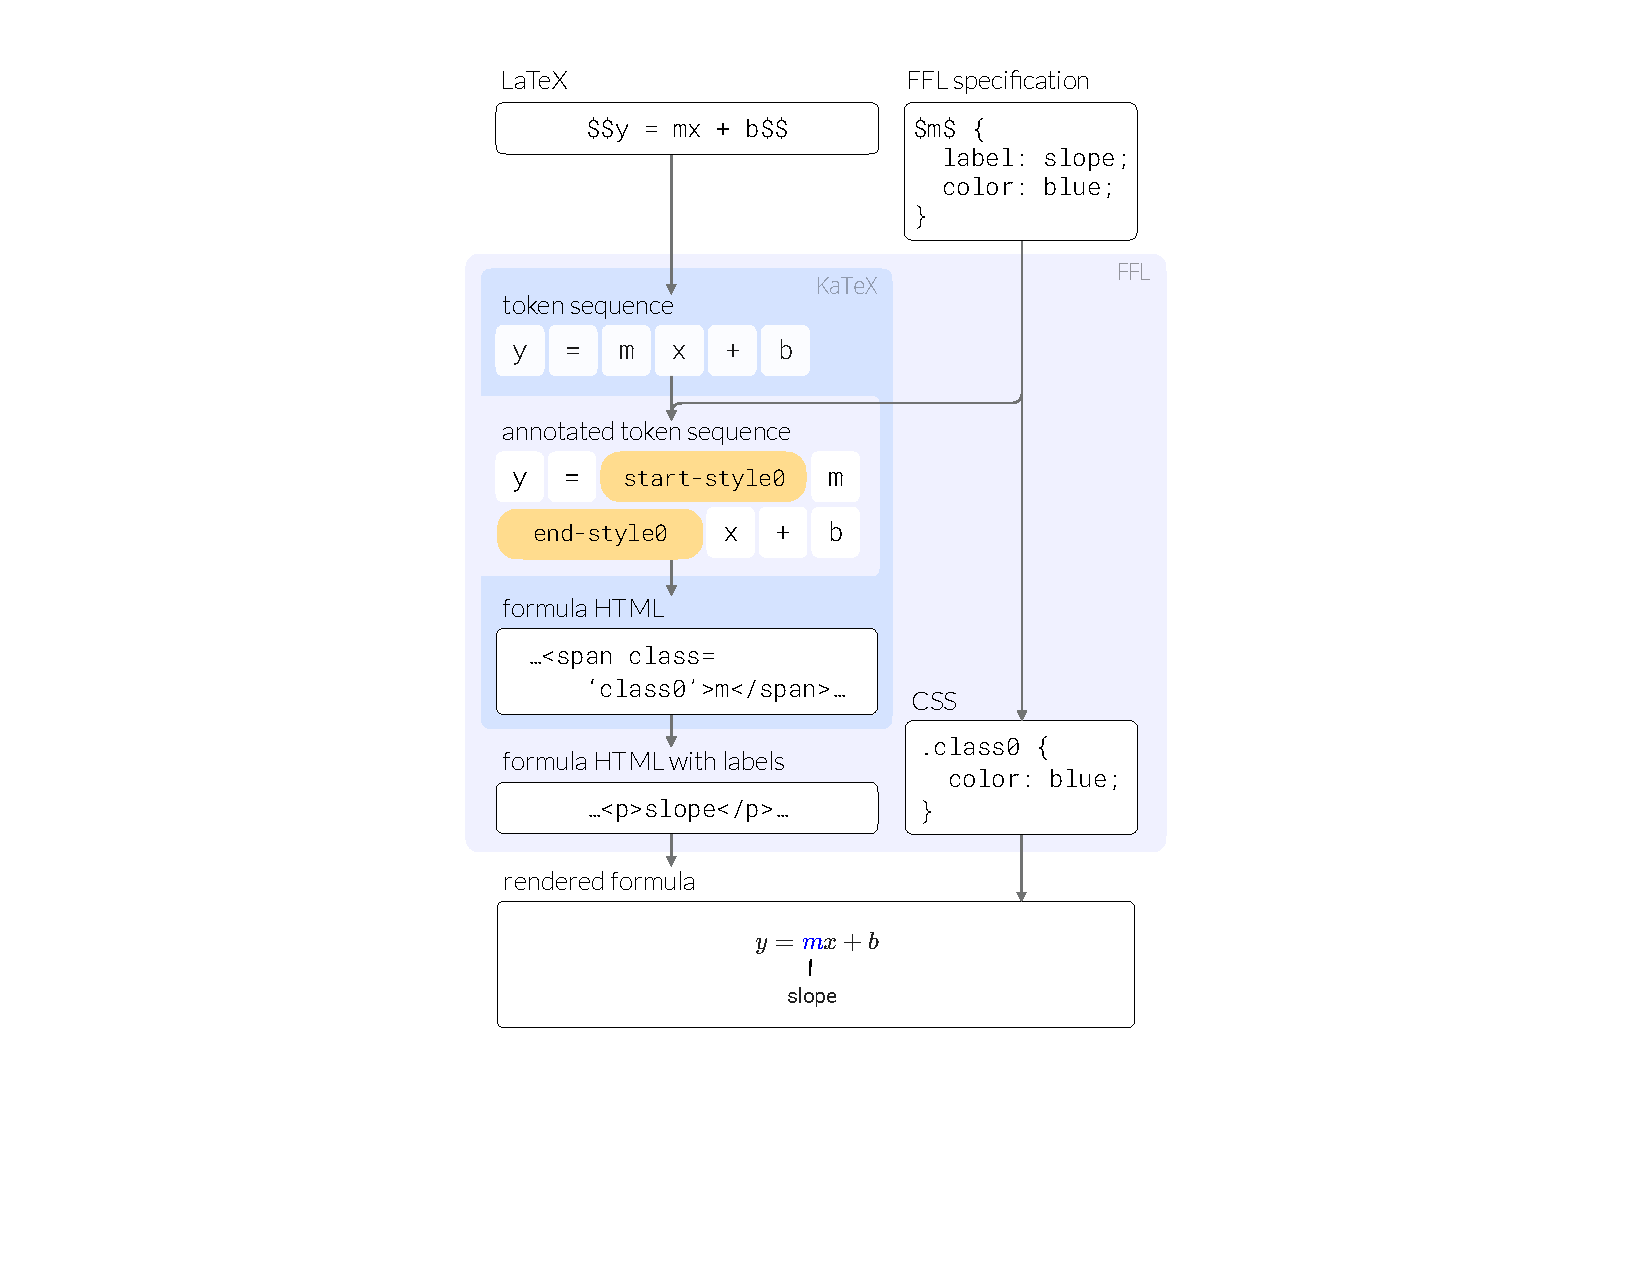
\includegraphics[width=.86\columnwidth]{figures/dataflow} 
    \caption{The generation of an augmented formula from LaTeX and an FFL style specification. \normalfont FFL wraps the  KaTeX library~\cite{tool:katex}, shimming itself into KaTeX's token parsing to detect and annotate expressions of interest. KaTeX generates an annotated HTML formula, which can be styled with CSS that FFL generates from its specification. FFL augments the generated HTML with labels by post-processing the generated HTML.}
    \Description{A decorative flowchart demonstrating how augmented formulas are generated from the LaTeX for a formula and an FFL style specification. The LaTeX math code and FFL style specification are passed into FFL, which then generates CSS from the FFL style specification and passes the LaTeX code to KaTeX, which FFL wraps. KaTeX tokenizes the LaTeX code and lets FFL insert marker tokens to indicate ranges where styles apply, linking the markers to generated CSS classes. KaTeX renders the token stream into HTML. FFL processes the HTML to add label elements. The HTML and CSS are rendered together as an augmented formula by the browser.}
    \label{fig:dataflow}
\end{figure}

\subsection{Parsing the FFL specification}
FFL markup is parsed using a custom parser for the FFL grammar. The parser was generated by Peggy~\cite{Peggy}, a PEG parser generator, from an FFL grammar that resembles a subset of CSS grammar.

\subsection{Matching LaTeX token sequences}
Next, the selectors are used to identify ranges of formula LaTeX that need to be augmented. To do this, we use KaTeX to lex both the selectors and the formula LaTeX into token sequences, with a small amount of parsing to normalize implicit groups. Then, we scan the LaTeX formula token stream for sub-sequences matching the selector, similarly tokenized by KaTeX. \zed{A segment and selector are considered matching if they contain a sequence of matching tokens. Literal tokens are considered matching if they are the same. The wildcards ``\texttt{?}'' and ``\texttt{*}'' match either a single or a sequence of tokens respectively. 
} The current implementation of sub-sequence search permits matching overlapping sub-sequences, and wildcard matches for the character and sequence wildcards.

Once a matching sub-sequence is found, KaTeX must be told to augment the characters in that sub-sequence. To do this, we insert special tokens before and after the sub-sequence. These special tokens instruct KaTeX to insert temporary \texttt{span} tags with a generated class name around the expression in the rendered formula HTML. While it inserts these special tokens, FFL creates a map from FFL selectors to the selector-specific class names, from which it builds a CSS style sheet that applies FFL styles (e.g., color, font weight) to the expression in the rendered HTML formula.

\zed{We implement the search for matching sub-sequences of tokens in a way that does not require changing KaTeX's implementation. Our approach is to handle matching in a custom KaTeX macro that we wrap around each formula. With KaTeX, macros are defined as JavaScript functions. When KaTeX expands a macro, it does so by calling the corresponding JavaScript function, passing the function the sequence of tokens found in the macro's arguments. We wrote a custom macro that, when expanded by KaTeX, takes the tokens of the formula, searches for matching sub-sequences, modifies those sub-sequences as described in the paragraphs above, and returns the modified tokens to KaTeX for further processing.}

\subsection{Applying styles}
Once KaTeX produces the HTML for a rendered formula, FFL traverses the HTML to associate styles with matched expressions. FFL searches for the previously inserted \texttt{span}s, removing them and applying generated CSS class names to the HTML elements between them. Then, it appends the generated CSS (including color and font weight) to a ``\texttt{style}'' element in the DOM, which has the effect of styling the matched elements in the expression.

\subsection{Drawing overlays and underlays}\label{sec:overlays}
Finally, all remaining kinds of augmentations collected during the HTML tree traversal are applied, including labels and background colors. Labels are drawn as relatively positioned HTML elements on the margins of the formula inside an SVG~\cite{tool:svg} element. Label positions are determined by locating the position and outer bounding box of all tokens in its corresponding expression. Label positions are adjusted to reduce overlap by Labella~\cite{tool:labella}. The formula is padded with additional space so that labels do not occlude the surrounding text. Background colors are implemented as relatively positioned boxes placed behind the corresponding expression; this implementation is necessary to support background colors for selections whose constituent elements have a joined area that differs from the rectangular bounding box of the whole expression to ensure that there is only one background box, rather than multiple overlapping boxes for each character element in the expression.

\subsection{Technical limitations}\label{tech-limitations}

Our current technical approach suffices for reifying the ideas behind FFL in a working tool. Here, we describe technical limitations that should be addressed to increase FFL's flexibility and robustness.

\paragraph{Behavior of sequence wildcard} One revelation from our development was that the \texttt{glob}-style ``\texttt{*}'' wildcard is not well-defined for strings with the inherent hierarchy of LaTeX formulas. The current behavior of ``\texttt{*}'' is to match any terminal token or group at the same group level as the ``\texttt{*}'' in the selector. This decision remains to be more closely examined.

\paragraph{Block styles}
For some styles, FFL transpiles directly to CSS. For others like background color, border, and padding, FFL requires custom solutions. The default approach of FFL is to apply a style to all tokens separately in an expression. Rather, block styling augmentations---like padding---should apply to an expression in whole. To overcome this brittleness for block styling, we believe future versions of FFL should use KaTeX's render to MathML~\cite{tool:mathml} instead of HTML; MathML contains structures that can be more easily detected and augmented for these styles, and has become mainstream into most major browsers earlier this year.

\paragraph{Performance}
\zed{Preliminary tests on a commodity laptop show that rendering a formula with FFL takes tens of milliseconds (i.e., 35ms to augment ``$x$'' in the linear regression formula from Section~\ref{Demo}). This runtime is imperceptible for single augmentations applied to single formulas. Our tests lead us to attribute latency to the time it takes FFL to insert augmentation markers into KaTeX's token stream: latency increases as more matches are found in the formula (e.g., it takes 50ms to augment expressions matching ``\texttt{\$*\$}'' in the same demo formula). As the number of augmentations and formulas grows, adjustments will be required (e.g., optimizations, parallelization) for FFL to continue to deliver instant feedback.}
